{\it This problem format was changed from library to interactive one }

A rod is either a horizontal or a vertical sequence of at least 2 consecutive grid cells.
Two rods, one horizontal and the other vertical, are placed on an $N \times N$ grid. In
picture below, the two rods are shown by X's. The rods may or may not be the same length;
furthermore, they may share a cell. If, from a diagram such as picture below, it is possible to interpret a cell, e.g. $(4,~4)$, as being in just one rod or in both rods, we make the interpretation that the cell is in both. Hence, the top cell of the vertical rod is $(4,~4)$ rather than $(5,~4)$.

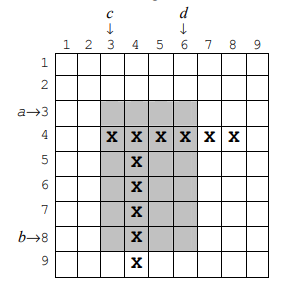
\includegraphics{pic.png}


Initially we do not know where the two rods are, and so your task is to write a program
to determine their locations. We call the horizontal rod ROD1, and the vertical rod
ROD2. Each grid cell is represented by a row/column pair $(r,~c)$, and the top left corner
of the grid is taken to be location $(1,~1)$. Each rod is represented as two cells, $<(r_1,~c_1), (r_2,~c_2)>$. In picture above ROD1 is $<(4,~3), (4,~8)>$ and ROD2 is $<(4,~4), (9,~4)>$.

To locate the rods, you can only use the interaction with jury's problem, which examines the rectangular region $[a,b]\times[c,d]$ (shaded region in the picture above), where $a \le b$ and c $\le d$ and responses whether at least one grid cell of either rod falls inside the query rectangle $[a,b]\times[c,d]$.

Your task is to write a program to discover the exact location of the rods using a limited number of interaction queries.
